\section{Industrial robots}

Industrial robots are automatically controlled, 
reprogrammable, general-purpose manipulating devices, 
programmable in three or more axes, 
which can be either fixed or mounted on a mobile 
platform for use in automation applications in an industrial 
environment.\cite{dagalakis1999industrial}\\
Robots can be used to weld, paint, assemble, 
disassemble,pick and place, pack and label, 
palletize.\cite{hagele2016industrial}
They can be an aid to material handling.\cite{hagele2016industrial}
\\In this project, due to the limitation of not having all types of industrial robots, we are only using arm type robots such as the KuKa KR3 to develop the required use case.
An arm robot, or better known as an \textbf{articulated robot}, is the most commonly used industrial robot. 
robot that resembles a human arm, hence the name robot arm or manipulating arm. 
manipulating arm. Articulated arms have multiple joints which allow them to 
which allow them to move in a variety of ways.\cite{hagele2016industrial}
\\
\begin{figure}[h]
    \centering
    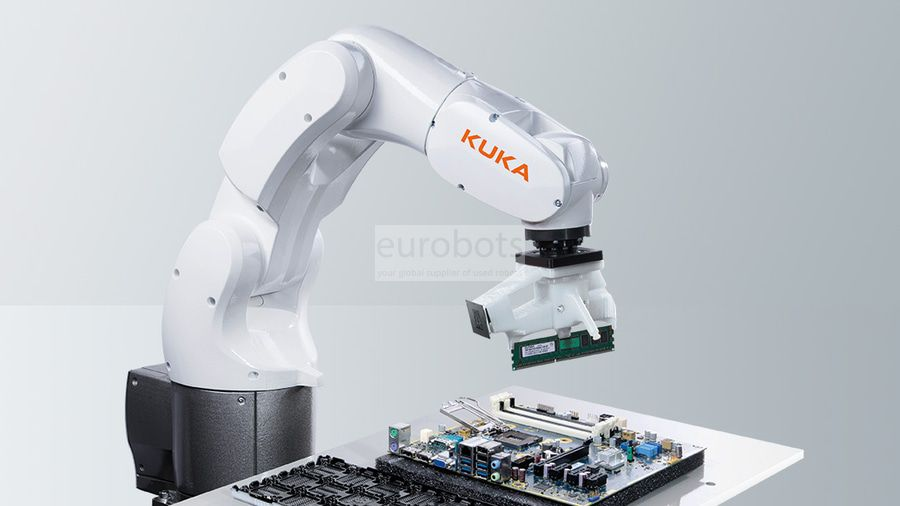
\includegraphics[width=0.9\textwidth]{KR_3_AGILUS}
    \caption{KuKa KR3 Cell}
    \label{fig:mesh4}
\end{figure}
